\paragraph*{Standard IT Balanced Scorecard}

Stabilisce il meccanismo per riportare obiettivi strategici e progessi IT alla
board.

Le \textit{dashboard} sono tutti quelli strumenti di gestione medio alti che
fanno capire i vari livelli (di liquidità, di sicurezza aziendale, ecc). Sono
indicatori semplici che sintetizzano strutture aziendali molto più complesse.

Ma come fanno le aziende a prendere le decisioni? Si sta andando sempre di più
verso decisioni basati sui dati. I rapporti contengono i dati, ma molto spesso
vengono visualizzati solamente i grafici di questi report.\\
\newline
Misure: statistiche costumer satisfaction (facile) e efficienza operazionale,
che però non è facile da misurare. Per esempio il numero di ticket chiusi in un
call center, o l'utilizzo di uno scontrino virtuale.

\begin{figure}[H]
        \begin{center}
                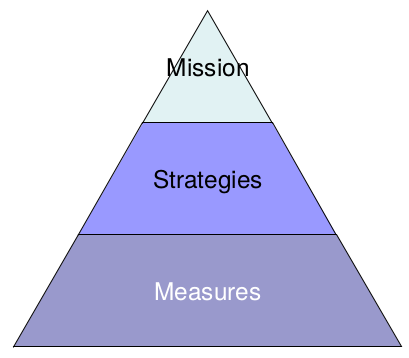
\includegraphics[scale=0.5]{res/img/measures}
        \end{center}
        \caption{Missione, strategie e misure.}
\end{figure}

Bisogna eccellere nei processi relativi al core business. Per controllare questi
processi si va a vedere l'analisi dei rischi, perché viene fatta su questi
processi.

\subsection{Organizzazione della sicurezza}

\subsubsection{Board of Directors}
In cima c'è il \textit{Board of Directors}, che fa la \textit{review} del
\textit{risk assessment} e del \textit{Business Impact Analysis}; definisce
anche la penalità per la non adesione alle policy.

A livello più basso c'è il Management Esecutivo (\textit{Executive Management}),
ossia chi definisce gli obiettivi di sicurezza e istituisce l'organizzazione
della sicurezza.

\subsubsection{Managers}

Il manager è colui che muove la società, che si sporca le mani azionando le leve
all'interno delle società.
Esistono differenti linee di management, principalmente ce ne sono quattro:
\begin{enumerate}
\item Collaboratore;
\item Lite Manager;
\item Lite Manager di secondo livello. Di solito i manager di questo livello
gestiscono in maniera effettiva da 5 a 7 persone;
\item Lite manager di terzo livello (detto anche \textit{executive}).
\end{enumerate}

\subsubsection{Security Steering Commitee}

Lo \textit{Steering commitee} è un comitato permanente composto da
rappresentanti senior delle funzionalità del business. Il suo ruolo è
assicurare l'allineamento del programma di sicurezza con gli obiettivi del
business.

\subsubsection{Chief Information Security Officer}

CISO è il penultimo passo prima di arrivare a quello che è l'obiettivo, ossia
diventare CIO. Altre posizioni sono il \textit{Chief Risk Officer} e il
\textit{Chief Compliance Officer}.

\subsubsection{IT Governance Committees}

\paragraph{IT Strategic Committee}

Si concentra sulla direzione e la strategia, aiuta il consiglio sulla strategia
e l'allineamento IT e ottimizza i costi IT e i rischi. Composta da membri del
consiglio (\textit{board}) e specialisti.

\subparagraph*{Main concerns}

\begin{itemize}
\item Allineamento dell'IT con il business;
\item Contributo dell'IT al business;
\item Esposizione e contenimento dei rischi;
\item Ottimizzazione dei costi IT;
\item Raggiungimento degli obiettivi strategici dell'IT.
\end{itemize}

\paragraph{IT Steering Committee}

Si concentra sull'implementazione, monitora i progetti correnti e decide le
spese per l'IT. Composto da business executives (utenti IT), CIO e consiglieri
chiave (IT, legale, audit, finanziario).

\subparagraph*{Main concerns}

\begin{itemize}
\item Prende decisioni sulla centralizzazione/decentralizzazione dell'IT e
assegna le responsabilità;
\item Fa raccomandazioni per i piani strategici;
\item Approva l'architettura IT;
\item Fa la review e approva i piani, i budget, le milestone e le priorità IT;
\item Monitora i piani dei maggiori progetti e fornisce le performance.
\end{itemize}

Cambiare architettura IT ottimizza il tempo di esecuzione dei processi, aiutando
il business (tempo di presa di decisioni minori, esecuzioni più rapide, ecc).

\subsubsection{Executive Mgmt Info Security Concerns}

\begin{itemize}
\item Ridurre responsabilità civili e legali legate alla privacy. La nuova
normativa sulla privacy europea prevede multe fino al 5\% del fatturato (non dei
profitti);
\item Fornisce le policy e gli standard per la leadership;
\item Controlla che i rischi siano a livelli accettabili;
\item Ottimizza le risorse limitate per la sicurezza;
\item Basa le decisioni su informazioni accurate;
\item Assegna le responsabilità per la salvaguardia dell'informazione;
\item Aumenta la fiducia e migliora la reputazione al di fuori
dell'organizzazione.
\end{itemize}


Le decisioni vengono continuamente prese in condizioni di incertezza, ma
comunque basandosi sui dati\footnote{Jeff Bezos, Il CEO di Amazon ha 
affermato che prende decisioni con un po' di incertezza, all'incirca 
quando ha l'80\% dell'informazione, ovvero quando si hanno abbastanza 
dati ma c'è un certo margine d'incertezza, questo perché aspettando il
90\% o il 100\% potrebbe essere troppo tardi.}.


\subsection{Esercizi}

Gli esercizi possono essere trovati nella Sezione \ref{esPG:SPP}
\newpage
\subsection{Road Map for Security}

\begin{figure}[h!]
        \begin{center}
                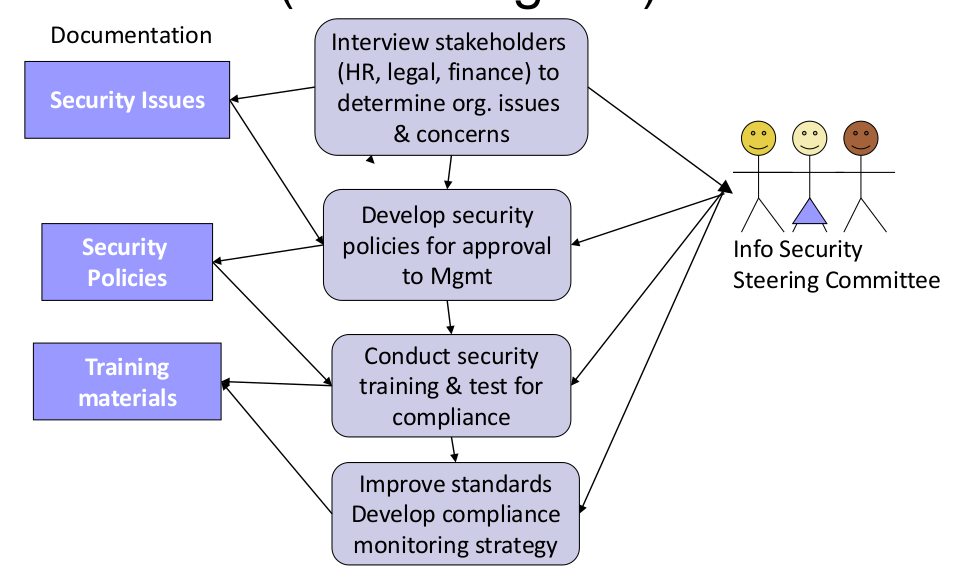
\includegraphics[scale=0.3]{res/img/roadmap}
        \end{center}
        \caption{Roadmap per la sicurezza.}
\end{figure}

\subsection{Security Relationships}

\begin{figure}[h!]
        \begin{center}
                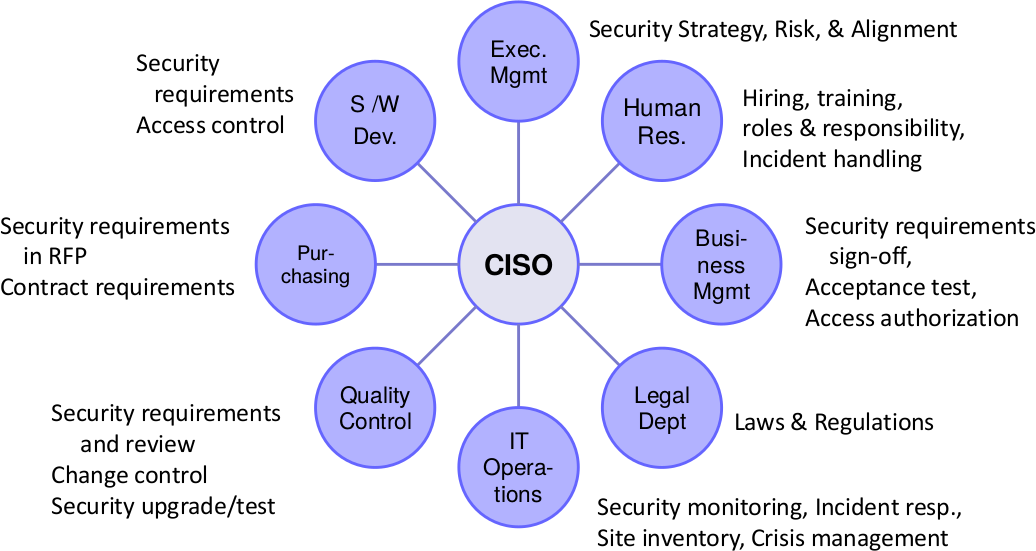
\includegraphics[scale=0.3]{res/img/relationships}
        \end{center}
        \caption{Relazioni nella sicurezza.}
\end{figure}


\subsection{Security Positions}

\subsubsection{Security Administrator}

\begin{itemize}
\item Alloca l'accesso ai dati sotto il proprietario dei dati stessi;
\item Prepara il programma di awareness per la sicurezza;
\item Testa la sicurezza del sistema;
\item Monitora le violazioni della sicurezza e attua misure correttive;
\item Revisiona e valuta le policy sulla sicurezza.
\end{itemize}

\subsubsection{Security Architect}

È una posizione senior, ci vuole tanta esperienza e viene pagata meglio del
security administrator, in quanto per fare il security architect bisogna
prima aver fatto l'amministratore.
Ci sarebbe anche il CTSO che capisce di una certa tecnologia e fa da tramite
con il business.

\begin{itemize}
\item Progetta topologie di rete, controllo degli accessi, policy sulla
sicurezza e standard sicuri;
\item Valuta le tecnologie per la sicurezza;
\item Lavora con chi si occupa di conformità, gestione del rischio e audit.
\end{itemize}

\paragraph{Security Architect: Control Analysis}

Se si vuole fare il \textit{security architect} la \textit{control analysis} è
importante.

\begin{figure}[h!]
        \begin{center}
                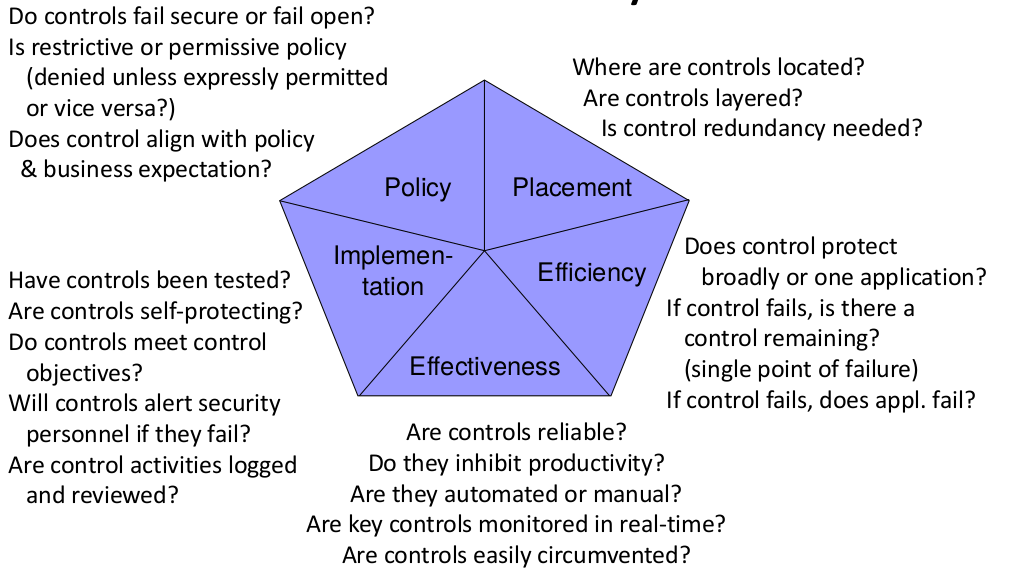
\includegraphics[scale=0.3]{res/img/penta}
        \end{center}
        \caption{Pentagono che illustra i diversi punti della control analysis.}
\end{figure}

\paragraph*{Esempi di policy per i documenti}

\textbf{Classificazione dei dati:} definisce le categorie di sicurezza dei dati,
la proprietà e la responsabilità.\\
\newline
\textbf{Policy accettabili di utilizzo:} descrive l'uso permesso delle risorse
IT.\\
\newline
\textbf{Policy per l'utente finale:} definisce l'utilizzo e i parametri degli
strumenti desktop.\\
\newline
\textbf{Policy di controllo degli accessi:} definiscono come i permessi
d'accesso sono definiti e allocati.\\
\newline
Dopo che le policy dei documenti sono create, devono essere ufficialmente
revisionate, aggiornate, diffuse e testate per la conformità.
